\section{Advanced Classification}
\label{sec:advanced_classification}

In this section, classification results are showcased for two
target variables: \texttt{averageRating} (properly binned into
5 classes), and \texttt{titleType} (with 6 classes).

\textcolor{red}{We then applied multiple classification models using the data as preprocessed previously (see Section~\ref{sec:understanding_preparation}).}   
\textcolor{blue}{The first target variable is \texttt{titleType}, which includes six categories: 
\textit{movie}, \textit{short}, \textit{tvEpisode}, \textit{tvSeries}, 
\textit{tvSpecial}, and \textit{video}. 
The classes are not equally distributed, with \textit{tvSpecial} and \textit{video} 
being significantly under-represented compared to the others. Entries labeled as \textit{videoGame} were removed from both the training and testing sets, 
as they were too few to be useful for classification. 
The remaining categories were merged into broader groups according to the following mapping: 
\textit{movie} and \textit{tvMovie} were grouped as \textit{movie}, 
\textit{short} and \textit{tvShort} were grouped as \textit{short}, 
\textit{tvSeries} and \textit{tvMiniSeries} were grouped as \textit{tvSeries}, 
while \textit{tvEpisode}, \textit{tvSpecial} and \textit{video} were left unchanged. 
All feature columns were standardized using a \textit{StandardScaler}. 
In addition, the variable \texttt{canHaveEpisodes} was removed prior to training, 
since it provides direct information about the target \texttt{titleType} 
and could therefore introduce data leakage.}
%-------------------------------------------------------------------------------

\subsection{Logistic Regression}
\label{subsec:logistic}

%-------------------------------------------------------------------------------
% titleType logistic
%-------------------------------------------------------------------------------
For the classification of the \texttt{titleType} variable, the target was transformed 
into numerical labels using \textit{LabelEncoder} and all numerical features were scaled 
with \texttt{StandardScaler} to ensure comparability across variables.

Since the problem is multi-class, we chose to present the results using the 
\textit{One-vs-Rest (OVR)} approach, which trains a binary classifier for each class. 
We also tested the \textit{multinomial} strategy, but it was significantly slower and 
produced comparable results, so OVR was selected for efficiency.

To optimize the model, a hyperparameter search was performed using 
\texttt{RandomizedSearchCV} with \texttt{StratifiedKFold} (5 folds), ensuring that the class 
distribution was preserved in each fold. The solver was set to \texttt{saga}, and the 
parameters tested included the regularization term $C$ (50 values logarithmically spaced 
between $10^{-3}$ and $10^2$), \texttt{penalty} (\texttt{l2} and \texttt{l1}), and 
\texttt{class\_weight} (\texttt{None} and \texttt{balanced}). The hyperparameter 
search was performed using \texttt{f1\_macro} as the scoring metric to balance 
performance across all classes. The best parameters selected by the search were 
\textbf{C = 6.16}, \textbf{penalty = l1}, and \textbf{class\_weight = balanced}.

For computational efficiency, the search was conducted on a 10\% stratified sample 
of the dataset, which was approximately representative of the original class distribution. The final 
model was then refitted on the full dataset using the best parameters. Evaluation on 
the test set was carried out using the confusion matrix, classification report, and 
one-vs-rest ROC curves for each class. The main performance metrics are summarized in 
Table~\ref{tab:logistic_report_t}, and the corresponding ROC curves are shown in 
Figure~\ref{fig:log_roc_curves_t}. 

\begin{figure}[ht]
    \centering
    \begin{minipage}{0.45\textwidth} % tabella a sinistra, 45% larghezza
    \centering
    \captionof{table}{Classification report for \texttt{titleType}}
    \label{tab:logistic_report_t}
    \small % riduce leggermente la dimensione del testo
    \begin{tabular}{lccc}
    \hline
    \textbf{Class} & \textbf{Precision} & \textbf{Recall} & \textbf{F1-score}\\
    \hline
    tvEpisode  & 0.89 & 0.88 & 0.89  \\
    movie      & 0.92 & 0.64 & 0.76  \\
    short      & 0.75 & 0.87 & 0.81  \\
    tvSeries   & 0.51 & 0.35 & 0.41  \\
    video      & 0.20 & 0.48 & 0.28  \\
    tvSpecial  & 0.07 & 0.49 & 0.11  \\
    \hline
    \textbf{Accuracy}    & \multicolumn{3}{c}{0.75} \\
    \textbf{Macro avg}   & 0.56 & 0.62 & 0.54  \\
    \textbf{Weighted avg}& 0.83 & 0.75 & 0.78  \\
    \hline
    \end{tabular}
    \end{minipage}
    \hfill
    \begin{minipage}{0.4\textwidth} 
    \centering
    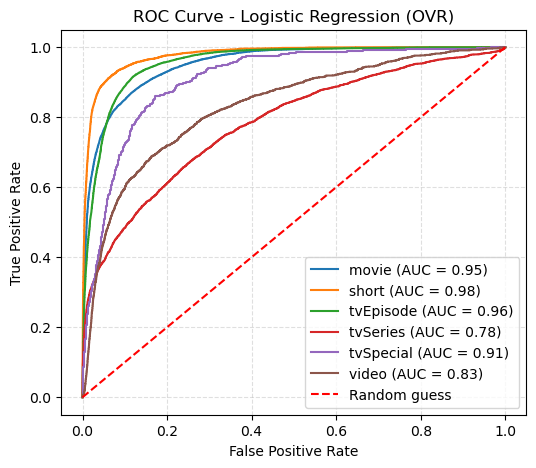
\includegraphics[width=\textwidth]{plotsss/log_roc_curves_t.png} 
    \captionof{figure}{ROC Logistic Regression}
    \label{fig:log_roc_curves_t} 
    \end{minipage}
    \end{figure}


From the results, we observe that the model achieves high performance for the 
\texttt{movie}, \texttt{short}, and \texttt{tvEpisode} classes, with F1-scores of 0.76, 
0.81, and 0.89, respectively. The model performs less well on \texttt{tvSeries}, 
\texttt{tvSpecial}, and \texttt{video}, likely due to lower support in the dataset.
Overall, the model reaches an accuracy of 0.75, 
a macro-average F1 of 0.54, and a weighted F1 of 0.78. These results highlight that 
while the model discriminates well among the more common classes, its performance is still
limited for rarer classes. 
This pattern is also reflected in the ROC curves shown in Figure~\ref{fig:log_roc_curves_t}, 
where the model clearly separates the more frequent classes, while discrimination is more limited 
for the less common categories.

% Coefficient analysis provided insight into the influence of each feature on the probability of belonging to different classes. 
% For each OVR classifier, the coefficients indicate how much a feature increases or decreases the probability of class membership 
% relative to the others. Globally, the most influential features were \texttt{budget}, \texttt{duration}, and \texttt{votes}. 
% Examining individual classes, for the \textit{film} class, \texttt{votes} and \texttt{budget} positively contribute, while 
% \texttt{duration} has a negative effect; for the \textit{series} class, \texttt{actors\_popularity} is positive, 
% while \texttt{budget} is negative; for the \textit{documentary} class, \texttt{duration} is positive, whereas
%  \texttt{votes} is negative. 
%  This interpretation was visualized through a coefficient heatmap and can also be summarized in a table of the top positive and negative features for each class.

Furthermore, coefficient analysis highlighted the main drivers for each class. Globally, \texttt{totalNomitations}, \texttt{numRegions}, and \texttt{runtimeMinutes} were most influential. 
For individual classes, for example, \texttt{movie} is positively influenced by \texttt{totalNomitations} but negatively by \texttt{genre3}; 
\texttt{short} is positively influenced by \texttt{totalNomitations} and negatively by \texttt{companiesNumber}; 
\texttt{tvEpisode} is positively influenced by \texttt{Europe} and negatively by \texttt{numRegions}.


%-------------------------------------------------------------------------------
% rating logistic 
%-------------------------------------------------------------------------------

Building upon the approach described for \texttt{titleType}, we trained a 
Logistic Regression model for the multi-class \texttt{rating\_class} variable. 
All numerical features were scaled and, in addition, the categorical variable 
\texttt{titleType} was included as a predictor and processed via \textit{One-Hot Encoding}.

Hyperparameters were optimized using again \texttt{RandomizedSearchCV} with \texttt{StratifiedKFold} (5 folds), 
performed on a 10\% stratified sample of the data for computational efficiency. 
The scoring metric was \texttt{f1\_macro}, and the search explored the same set of parameters used for \texttt{titleType}. 
The optimal configuration was found to be: \textbf{C = 0.08}, \textbf{penalty = l2 }, and \textbf{class\_weight = balanced}.

The best parameters were then used to fit the model on the full dataset, and evaluation on the test set was carried out. 

% From the results, we observe that the model shows limited overall performance on the \texttt{rating\_class} test set,
% achieving an accuracy of 0.27, a macro-average F1 of 0.25, and a weighted F1 of 0.27. 
% Performance varies considerably across classes: the model predicts relatively better the mid-range ratings 
% (\texttt{[7, 8)}), with an F1-score of 0.40, while predictions for the lower and higher extremes 
% (\texttt{[1, 5)}, \texttt{[9, 10)}) are notably weaker. 


The results for the \texttt{rating\_class} target are reported in 
Table~\ref{tab:logistic_report_rating} and Figure~\ref{fig:log_roc_curves_rating}. 
Overall, the model shows limited predictive ability 
(\textbf{accuracy = 0.27}, \textbf{macro F1 = 0.25}), with marked variability across classes. 
The extreme intervals, \texttt{[1,5)} and \texttt{[9,10)}, are detected with relatively high recall 
(0.44 and 0.57), but their low precision yields modest F1-scores. 
In contrast, the central ranges, which dominate the distribution, prove more difficult to classify: 
\texttt{[6,7)} reaches only 0.13 in F1, while \texttt{[7,8)} performs slightly better at 0.40. 

Regarding ROC curves: discrimination is stronger for the extreme categories 
(AUCs of 0.75 and 0.76), whereas separability is weaker in the central intervals 
(\texttt{[6,7)}: 0.60, \texttt{[7,8)}: 0.64). 
This suggests that Logistic Regression tends to identify outlier ratings more effectively, 
while struggling to capture subtle differences in the middle of the rating scale.

 

\begin{figure}[ht]
    \centering
    \begin{minipage}{0.45\textwidth}
        \centering
        \captionof{table}{Classification report for \texttt{rating\_class}}
        \label{tab:logistic_report_rating}
        \small
        \begin{tabular}{lccc}
        \hline
        \textbf{Class} & \textbf{Precision} & \textbf{Recall} & \textbf{F1-score}\\
        \hline
        \texttt{[1, 5)}   & 0.20 & 0.44 & 0.27 \\
        \texttt{[5, 6)}   & 0.26 & 0.32 & 0.29 \\
        \texttt{[6, 7)}   & 0.39 & 0.08 & 0.13 \\
        \texttt{[7, 8)}   & 0.48 & 0.34 & 0.40 \\
        \texttt{[8, 9)}   & 0.25 & 0.22 & 0.24 \\
        \texttt{[9, 10)}  & 0.09 & 0.57 & 0.16 \\
        \hline
        \textbf{Accuracy}    & \multicolumn{3}{c}{0.27} \\
        \textbf{Macro avg}   & 0.28 & 0.33 & 0.25 \\
        \textbf{Weighted avg}& 0.35 & 0.27 & 0.27 \\
        \hline
        \end{tabular}
        \end{minipage}
    \hfill
    \begin{minipage}{0.4\textwidth} 
    \centering
    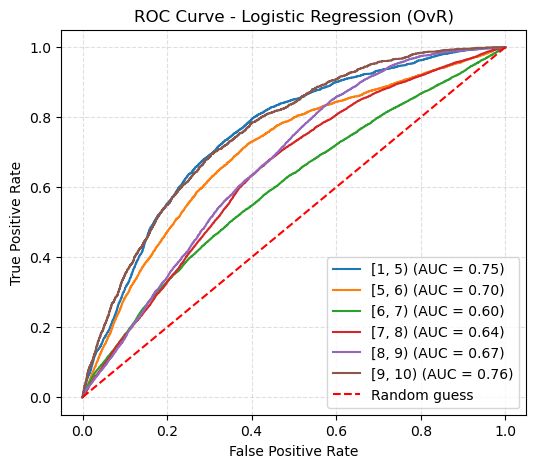
\includegraphics[width=\textwidth]{plotsss/log_roc_curves_rating.png} 
    \captionof{figure}{ROC curves for \texttt{rating\_class} (OvR)}
    \label{fig:log_roc_curves_rating} 
    \end{minipage}
\end{figure}





%-------------------------------------------------------------------------------
\subsection{Support Vector Machines}
\label{subsec:svm}

%-------------------------------------------------------------------------------
% titleType
%-------------------------------------------------------------------------------

We applied Support Vector Machines (SVM) to the \texttt{titleType} classification task.
Both linear and non-linear kernels were explored in order to evaluate how decision boundary complexity influences predictive performance.

The first experiment used a Linear SVM trained on the full dataset.  
A grid search with five-fold cross validation was carried out on the parameters 
$C \in \{0.01, 0.1, 1, 10, 100\}$ and $max\_iter \in \{1000, 5000, 10000\}$. 
The optimal configuration, with $C=100$ and $max\_iter=1000$, achieved a test accuracy of 0.81. 
While precision and recall were high for majority classes (\textit{movie}, \textit{short}, \textit{tvEpisode}), 
the classifier failed on \textit{tvSeries}, \textit{tvSpecial}, and \textit{video}, 
indicating that a linear decision boundary is insufficient for this problem.  

Non-linear kernels were then evaluated. 
A grid search was first performed on a stratified 10\% subset of the training set to efficiently explore a wide range of hyperparameters for each kernel, 
since a full search on the complete dataset would have been computationally prohibitive. 
For the RBF kernel, $C$ was varied from 0.01 to 1000 and $\gamma$ between \texttt{scale} and \texttt{auto}. 
The polynomial kernel was tested with $C$ from 0.01 to 100, degree 2--4, $\gamma$ as \texttt{scale} or \texttt{auto}, and \texttt{coef0} 0 or 1. 
The sigmoid kernel was explored over $C$ 0.01--100, $\gamma$ \texttt{scale}/\texttt{auto}, and \texttt{coef0} 0 or 1. 
\textcolor{blue}{Remember to fix C!}

The best configuration for each kernel, reported in Table~\ref{tab:svm_results}, was then retrained on the full dataset and evaluated on the test set. 
Both RBF and polynomial kernels reached approximately 0.90 test accuracy, substantially outperforming the linear baseline and sigmoid. 
The RBF kernel was selected as the reference non-linear model due to slightly more stable results and improved recall on the under-represented classes.


ROC curves were used to evaluate class separability 
%(Figure~\ref{fig:roc_four}),
showing excellent separation for majority classes, although minority categories remained problematic. 

\textcolor{red}{I will change the text and explain the figures better.}

To address class imbalance, the RBF kernel was retrained with \texttt{class\_weight=balanced}, 
which penalizes misclassification of under-represented classes. 
This model reached a slightly lower overall accuracy of 0.84, 
but recall for \textit{tvSpecial} and \textit{video} improved, providing a more equitable classification across categories.  
Confusion matrices (Figure~\ref{fig:rbf_balanced_two}) 
illustrate that \textit{tvSpecial} and \textit{video} ...  
Analysis of the support vectors confirmed this effect. 
In the unbalanced RBF, nearly all points of minority classes became support vectors, 
while in the balanced model the total number of support vectors increased and was more evenly distributed across classes, 
indicating a more complex but fairer decision function. 

Table~\ref{tab:svm_results} summarizes the main results, including the parameters used for each kernel and the corresponding test performance. 


\begin{table}[h]
\centering
\caption{Comparison of SVM models on the IMDb classification task.}
\label{tab:svm_results}
\begin{tabular}{lccc}
\hline
\textbf{Model} & \textbf{Best Params (main)} & \textbf{Test Accuracy} & \textbf{Macro F1-score} \\
\hline
Linear SVM & $C=100$, $max\_iter=1000$ & 0.81 & 0.45 \\
RBF kernel & $C=10$, $\gamma=\text{scale}$ & 0.90 & 0.64 \\
Polynomial kernel & $C=10$, degree=3, $\gamma=\text{auto}$ & 0.90 & 0.64 \\
Sigmoid kernel & $C=0.1$, $\gamma=\text{auto}$ & 0.65 & 0.36 \\
RBF (balanced) & $C=10$, $\gamma=\text{scale}$, balanced & 0.84 & 0.65 \\
\hline
\end{tabular}
\end{table}
    
% --- First figure: four ROC curves side by side ---
\begin{figure}[h]
    \centering
    \begin{subfigure}[b]{0.24\textwidth}
        \centering
        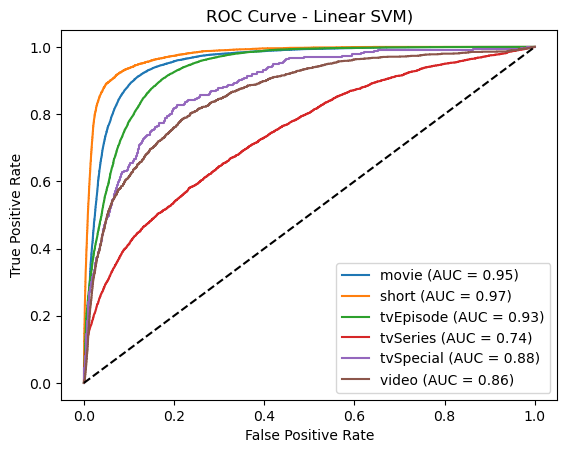
\includegraphics[width=\textwidth]{plotsss/roc_linear.png}
        \caption{Linear SVM}
        \label{fig:roc_linear}
    \end{subfigure}
    \begin{subfigure}[b]{0.24\textwidth}
        \centering
        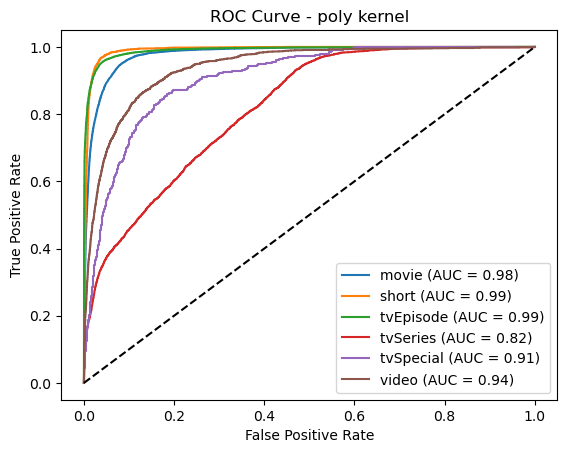
\includegraphics[width=\textwidth]{plotsss/roc_poly.png}
        \caption{Polynomial kernel}
        \label{fig:roc_poly}
    \end{subfigure}
    \begin{subfigure}[b]{0.24\textwidth}
        \centering
        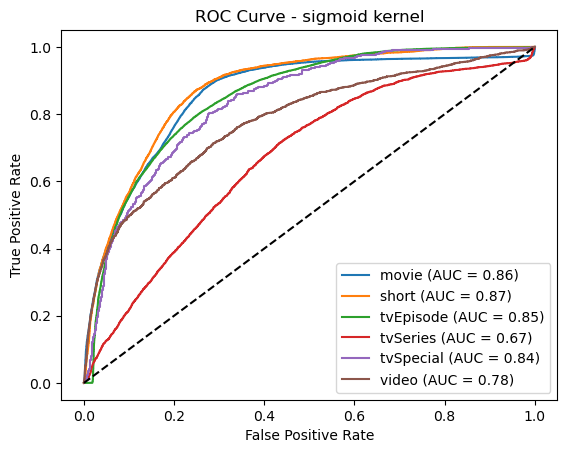
\includegraphics[width=\textwidth]{plotsss/roc_sigmoid.png}
        \caption{Sigmoid kernel}
        \label{fig:roc_sigmoid}
    \end{subfigure}
    \begin{subfigure}[b]{0.24\textwidth}
        \centering
        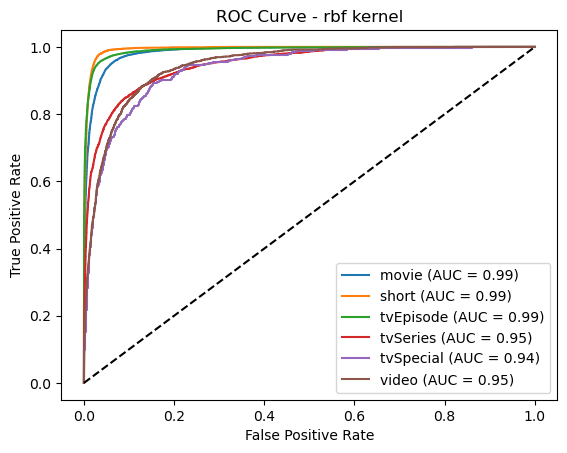
\includegraphics[width=\textwidth]{plotsss/roc_rbf.png}
        \caption{RBF kernel}
        \label{fig:roc_rbf}
    \end{subfigure}
    \caption{...}  
    \label{fig:roc_four}
\end{figure}

% --- Second figure: confusion matrix and ROC for RBF balanced ---
\begin{figure}[h]
    \centering
    \begin{subfigure}[b]{0.47\textwidth}
        \centering
        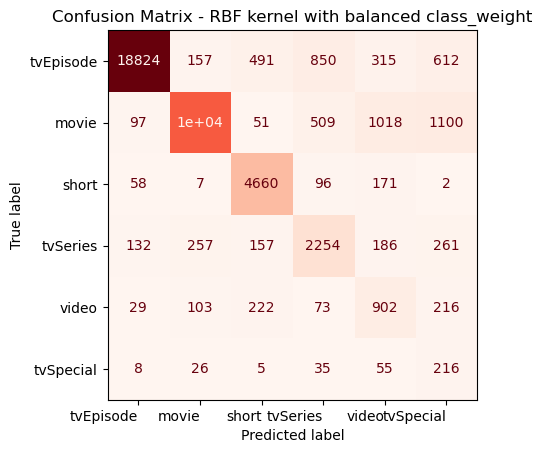
\includegraphics[width=\textwidth]{plotsss/new_cm_rbf_balanced.png}
        \caption{Confusion Matrix RBF balanced}
        \label{fig:cm_rbf_balanced}
    \end{subfigure}
    \begin{subfigure}[b]{0.43\textwidth}
        \centering
        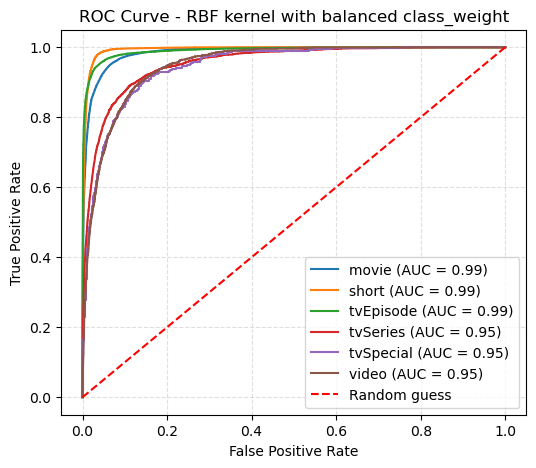
\includegraphics[width=\textwidth]{plotsss/new_roc_rbf_balanced.png}
        \caption{ROC RBF balanced}
        \label{fig:roc_rbf_balanced}
    \end{subfigure}
    \caption{Confusion Matrix and ROC Curve for the SVM (kernel rbf and balanced class weight) on the \texttt{titleType} classification task.}  
    \label{fig:rbf_balanced_two}
\end{figure}

% In conclusion, non-linear kernels were clearly superior to the linear SVM, 
% with RBF and polynomial achieving comparable accuracy. 
% The RBF kernel with balanced class weights provided the best compromise, 
% maintaining strong performance on majority classes while improving recognition of minority ones.

%-------------------------------------------------------------------------------
% rating
%-------------------------------------------------------------------------------

We also applied SVM to the \texttt{averageRating} classification task.
The same kernels and hyperparameter search strategies were used as for \texttt{titleType}.

We then applied the same methodology to the \texttt{rating} classification task.
% Here the output space is ordinal, ranging from $[1,6)$ to $[9,10)$, with strong class imbalance: 
% intermediate ranges are frequent, while extreme categories are under-represented.

A Linear SVM was first tested using the same hyperparameter grid as before.
The best configuration ($C=100$, $max_iter=1000$) achieved only 0.37 accuracy 
and a macro F1-score of 0.28, confirming (perchè confirming?) that a linear decision 
boundary is inadequate for this task.

We therefore moved to non-linear kernels.
As for the previous experiment, a grid search on a stratified 10\% subset of 
the training set was conducted. The optimal configurations were $C=10$, $\gamma=\text{auto}$ 
for the RBF kernel, $C=10$, degree=2, $\gamma=\text{scale}$, $\text{coef0}=1$ for the polynomial 
kernel, and $C=0.1$, $\gamma=\text{auto}$, $\text{coef0}=0$ for the sigmoid kernel.
These models were then retrained on the full dataset.

Results were generally lower than in the \texttt{titleType} task, with the RBF and polynomial 
kernels both reaching around 0.42 macro F1, while sigmoid performed substantially worse (macro F1 $\approx 0.36$).
Confusion matrices showed that the models correctly identified the most populated bins, but failed on the tails 
(\textit{[1,6)} and \textit{[9,10)}).

Finally, to mitigate imbalance, the RBF kernel was retrained with \texttt{$class\_weight=balanced$}.
This increased recall on minority classes, at the cost of a slight drop in overall accuracy, 
producing a fairer but more complex decision function.
However, even the balanced model struggled to capture the extremes of the rating distribution.


\subsection{Ensemble methods}
Boosting and Random Forest models were trained on the classification,
while being optimized via Stratified Randomized Search with 5-fold
cross-validation over a predefined hyperparameter space.\\

% rf
% RandomForestClassifier(max_depth=19, max_features=0.7361716094628554,
                    %    min_samples_leaf=3, min_samples_split=4, n_estimators=42,
                    %    n_jobs=-1, random_state=42)
% precision    recall  f1-score   support

%            0       0.56      0.60      0.58      9717
%            1       0.44      0.34      0.39     11114
%            2       0.48      0.68      0.56     14674
%            3       0.46      0.27      0.34      7640
%            4       0.60      0.16      0.25      1715

%     accuracy                           0.49     44860
%    macro avg       0.51      0.41      0.42     44860
% weighted avg       0.49      0.49      0.47     44860


% adaboost
% best_params = {'estimator__max_depth': 10, 'estimator__min_samples_leaf': 16, 'estimator__min_samples_split': 16, 'learning_rate': 0.46606998421703594, 'n_estimators': 56}
% precision    recall  f1-score   support

%            0       0.48      0.40      0.43      9717
%            1       0.33      0.31      0.32     11114
%            2       0.42      0.55      0.47     14674
%            3       0.31      0.28      0.29      7640
%            4       0.44      0.11      0.18      1715

%     accuracy                           0.39     44860
%    macro avg       0.40      0.33      0.34     44860
% weighted avg       0.39      0.39      0.38     44860

For the \texttt{averageRating} classification task, the best
hyperparameters for the Random Forest model were:
\texttt{n\_estimators=42}, \texttt{max\_depth=19}, \texttt{min\_samples\_split=4},
\texttt{min\_samples\_leaf=3}, \texttt{max\_features=0.74},
\texttt{criterion='gini'}, \texttt{class\_weight=None}.

For the AdaBoost model, the best hyperparameters were:
\texttt{n\_estimators=56}, \texttt{learning\_rate=0.47},
\texttt{estimator\_\_max\_depth=10},
\texttt{estimator\_\_min\_samples\_split=16},
\texttt{estimator\_\_min\_samples\_leaf=16}.

The table below summarizes the classification report for both models.
\begin{table}[H]
    \centering
    \label{tab:classification_report}
    \begin{tabular}{lccccc}
    \hline
    \textbf{Model} & \textbf{Accuracy} & \textbf{Macro Precision} & \textbf{Macro Recall} & \textbf{Macro F1-score} \\
    \hline
    Random Forest & 0.49 & 0.51 & 0.41 & 0.42 \\
    AdaBoost & 0.39 & 0.40 & 0.33 & 0.34 \\
    \hline
    \end{tabular}
    \caption{Performances of the models on the \texttt{averageRating} classification task.}
\end{table}

The Random Forest model outperforms AdaBoost in all metrics.
The biggest difference is found in the recall.

Figure~\ref{fig:cm_rf} and Figure~\ref{fig:cm_ab} show the confusion matrices
for the models.
\begin{figure}[H]
    \centering
    \begin{subfigure}[b]{0.45\textwidth}
        \centering
        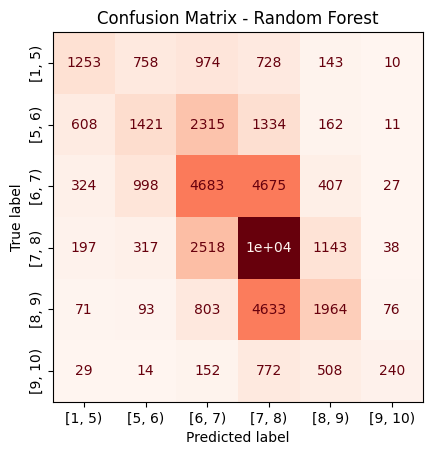
\includegraphics[width=\textwidth]{plotsss/conf_matr_rf_rating}
        \caption{Confusion Matrix - Random Forest}
        \label{fig:cm_rf}
    \end{subfigure}
    \hfill
    \begin{subfigure}[b]{0.45\textwidth}
        \centering
        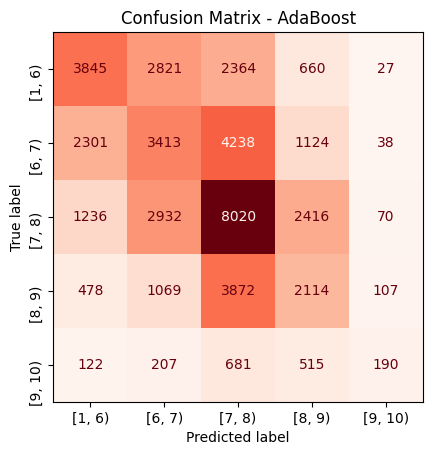
\includegraphics[width=\textwidth]{plotsss/conf_matr_boost_rating}
        \caption{Confusion Matrix - AdaBoost}
        \label{fig:cm_ab}
    \end{subfigure}
    \caption{Confusion matrices for the ensemle models on the \texttt{averageRating} classification task.}
    \label{fig:cm_comparison}
\end{figure}

From these, it can be seen why the recall is much lower for AdaBoost,
with regards to Random Forest: the former tends to classify less
aggressively as the most represented class.
It's also worth noting that Random Forest tends to assign
most of the misclassifications to the adjacent classes,
while AdaBoost spreads them more evenly across all classes.

Figures ~\ref{fig:roc_rf} and ~\ref{fig:roc_ab} show the ROC curves
for the two models.
\begin{figure}[h]
    \centering
    \begin{subfigure}[b]{0.45\textwidth}
        \centering
        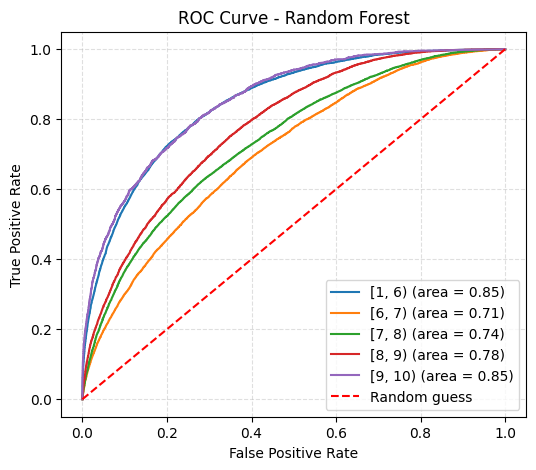
\includegraphics[width=\textwidth]{plotsss/roc_rf_rating}
        \caption{ROC Curve - Random Forest}
        \label{fig:roc_rf}
    \end{subfigure}
    \hfill
    \begin{subfigure}[b]{0.45\textwidth}
        \centering
        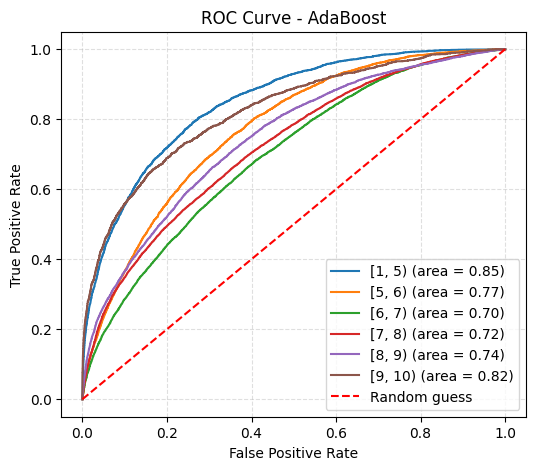
\includegraphics[width=\textwidth]{plotsss/roc_boost_rating}
        \caption{ROC Curve - AdaBoost}
        \label{fig:roc_ab}
    \end{subfigure}
    \caption{ROC curves for the ensemble models on the \texttt{averageRating} classification task.}
    \label{fig:roc_comparison}
\end{figure}
From these representations, it can be seen that AdaBoost has
poorer performances in all classes, but especially struggles
with the under-represented ones, which lead to the biggest
difference in Area Under The Curve (AUC).


On the \texttt{titleType} classification task, the best hyperparameters
obtained for the Random Forest model were:
% {'class_weight': None, 'criterion': 'gini', 'max_depth': 19, 'max_features': 0.7361716094628554, 'min_samples_leaf': 3, 'min_samples_split': 4, 'n_estimators': 42}
\texttt{n\_estimators=42}, \texttt{max\_depth=19}, \texttt{min\_samples\_split=4},
\texttt{min\_samples\_leaf=3}, \texttt{max\_features=0.74},
\texttt{criterion='gini'}, \texttt{class\_weight=None}.
% precision    recall  f1-score   support

%        movie       0.91      0.95      0.93     12947
%        short       0.93      0.96      0.95      4994
%    tvEpisode       0.96      0.98      0.97     21249
%     tvSeries       0.77      0.70      0.73      3247
%    tvSpecial       0.69      0.26      0.38       345
%        video       0.77      0.42      0.55      1545

%     accuracy                           0.92     44327
%    macro avg       0.84      0.71      0.75     44327
% weighted avg       0.92      0.92      0.92     44327


% adaboost
% Best parameters found for AdaBoost: {'estimator__max_depth': 10, 'estimator__min_samples_leaf': 16, 'estimator__min_samples_split': 16, 'learning_rate': 0.46606998421703594, 'n_estimators': 56}
For the AdaBoost model, the best hyperparameters were:
\texttt{n\_estimators=56}, \texttt{learning\_rate=0.47},
\texttt{estimator\_\_max\_depth=10},
\texttt{estimator\_\_min\_samples\_split=16},
\texttt{estimator\_\_min\_samples\_leaf=16}.
%            precision    recall  f1-score   support

%        movie       0.87      0.95      0.91     12947
%        short       0.92      0.95      0.94      4994
%    tvEpisode       0.96      0.97      0.96     21249
%     tvSeries       0.75      0.63      0.68      3247
%    tvSpecial       0.73      0.09      0.16       345
%        video       0.70      0.32      0.44      1545

The table below summarizes the classification report for both models.
\begin{table}[H]
    \centering
    \label{tab:classification_report}
    \begin{tabular}{lccccc}
    \hline
    \textbf{Model} & \textbf{Accuracy} & \textbf{Macro Precision} & \textbf{Macro Recall} & \textbf{Macro F1-score} \\
    \hline
    Random Forest & 0.92 & 0.84 & 0.71 & 0.75 \\
    AdaBoost & 0.90 & 0.82 & 0.65 & 0.68 \\
    \hline
    \end{tabular}
    \caption{Performances of the models on the \texttt{titleType} classification task.}
\end{table}

Figure~\ref{fig:cm_rf} and Figure~\ref{fig:cm_ab} show the confusion matrices
for the models.

\begin{figure}[H]
    \centering
    \begin{subfigure}[b]{0.49\textwidth}
        \centering
        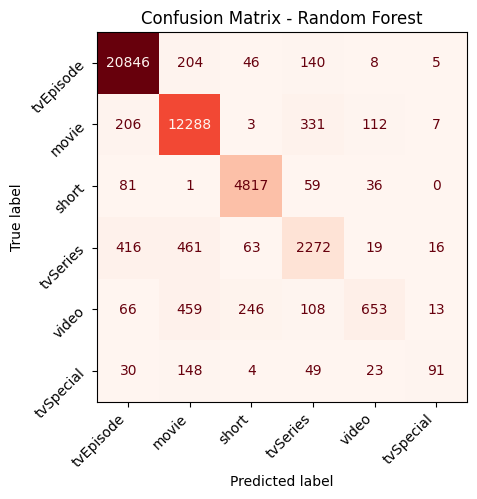
\includegraphics[width=\textwidth]{plotsss/conf_matr_rf_titletype}
        \caption{Confusion Matrix - Random Forest}
        \label{fig:cm_rf}
    \end{subfigure}
    \hfill
    \begin{subfigure}[b]{0.49\textwidth}
        \centering
        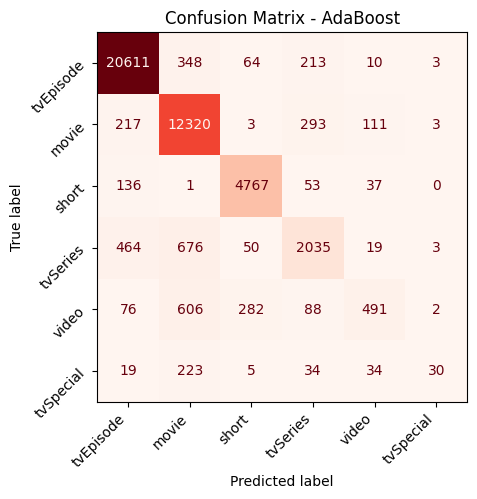
\includegraphics[width=\textwidth]{plotsss/conf_matr_boost_titletype}
        \caption{Confusion Matrix - AdaBoost}
        \label{fig:cm_ab}
    \end{subfigure}
    \caption{Confusion matrices for the ensemle models on the \texttt{titleType} classification task.}
    \label{fig:cm_comparison}
\end{figure}
Both models perform well on the first four classes, while struggling
with /texttt{video} and /texttt{tvSpecial}, which are the most
under-represented classes. In general, the two models show similar
performances, with Random Forest generally outperforming AdaBoost
by a slight margin.
Contrary to the results, the models base their decisions
on different feature importances: while Random Forest assigns over
half of the importance to \texttt{runtimeMinutes},
AdaBoost spreads the importance evenly across multiple features,
with the top being \texttt{runtimeMinutes} with around 15\%.


The ROC curves for the two models are shown in Figure~\ref{fig:roc_rf} and
Figure~\ref{fig:roc_ab}.
\begin{figure}[h]
    \centering
    \begin{subfigure}[b]{0.45\textwidth}
        \centering
        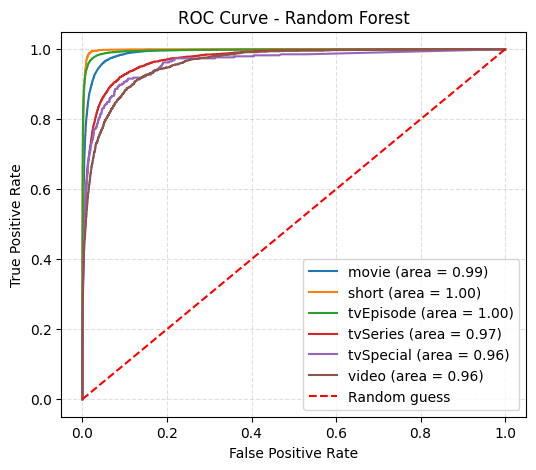
\includegraphics[width=\textwidth]{plotsss/roc_rf_titletype}
        \caption{ROC Curve - Random Forest}
        \label{fig:roc_rf}
    \end{subfigure}
    \hfill
    \begin{subfigure}[b]{0.45\textwidth}
        \centering
        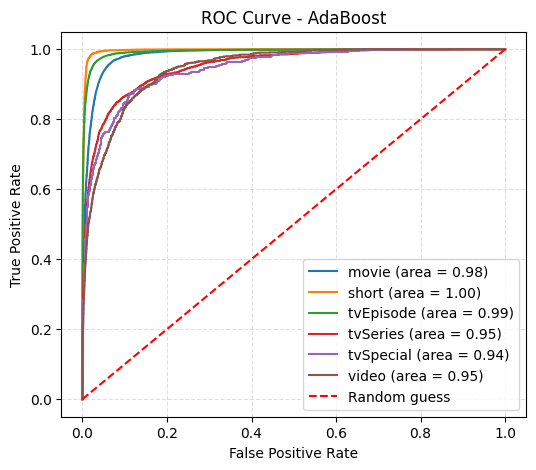
\includegraphics[width=\textwidth]{plotsss/roc_boost_titletype}
        \caption{ROC Curve - AdaBoost}
        \label{fig:roc_ab}
    \end{subfigure}
    \caption{ROC curves for the ensemble models on the \texttt{titleType} classification task.}
    \label{fig:roc_comparison}
\end{figure}

Again, similar performances are observed. The biggest difference
seems to be found in the under-represented classes, which seem to
have a bigger difference in Area Under The Curve (AUC).




\subsection{Neural Networks}

\begin{figure}
    \centering
    \begin{subfigure}[b]{0.48\textwidth}
        \centering
        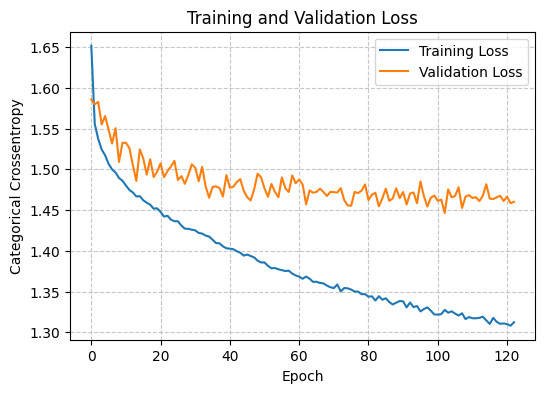
\includegraphics[width=\textwidth]{plotsss/loss_rating.png}
        \caption{Loss - Neural Network}
        \label{fig:loss_nn_rating}
    \end{subfigure}
    \hfill
    \begin{subfigure}[b]{0.48\textwidth}
        \centering
        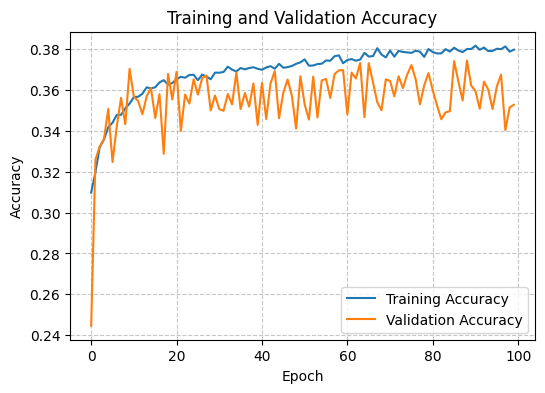
\includegraphics[width=\textwidth]{plotsss/accuracy_rating.png}
        \caption{Accuracy - Neural Network}
        \label{fig:accuracy_nn_rating}
    \end{subfigure}
    \caption{Training and validation loss and accuracy for the neural network on the \texttt{averageRating} classification task.}
    \label{fig:nn_performance_rating}
\end{figure}

\begin{figure}
    \centering
    \begin{subfigure}[b]{0.44\textwidth}
        \centering
        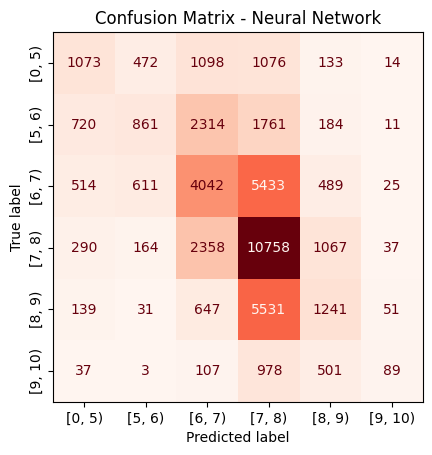
\includegraphics[width=\textwidth]{plotsss/cm_nn_rating.png}
        \caption{Confusion Matrix - Neural Network}
        \label{fig:cm_nn_rating}
    \end{subfigure}
    \hfill
    \begin{subfigure}[b]{0.52\textwidth}
        \centering
        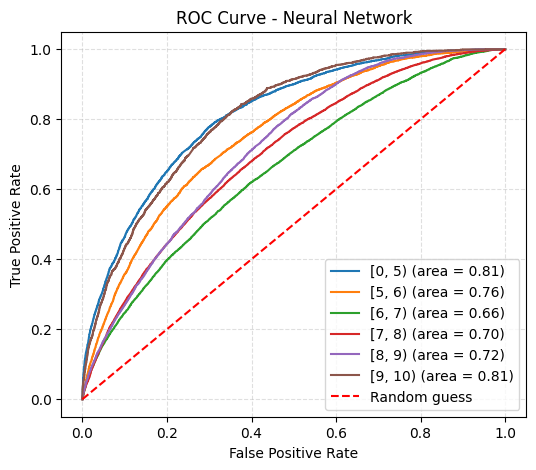
\includegraphics[width=\textwidth]{plotsss/roc_nn_rating.png}
        \caption{ROC Curve - Neural Network}
        \label{fig:roc_nn_rating}
    \end{subfigure}
    \caption{Confusion Matrix and ROC Curve for the Neural Network on the \texttt{averageRating} classification task.}
    \label{fig:cm_nn_rating}
\end{figure}


% titletype task

\begin{figure}
    \centering
    \begin{subfigure}[b]{0.48\textwidth}
        \centering
        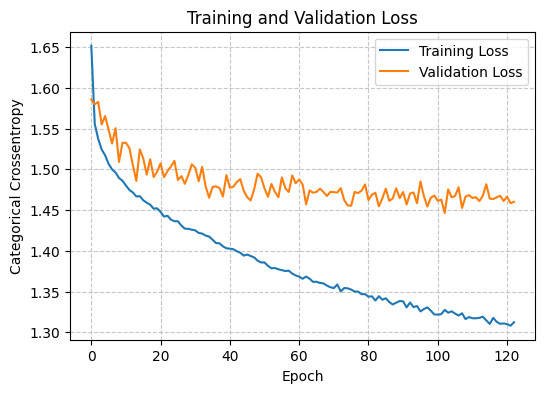
\includegraphics[width=\textwidth]{plotsss/loss_titletype.png}
        \caption{Loss - Neural Network}
        \label{fig:loss_nn_titletype}
    \end{subfigure}
    \hfill
    \begin{subfigure}[b]{0.48\textwidth}
        \centering
        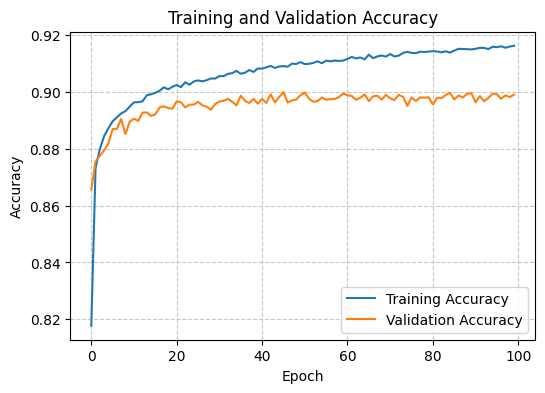
\includegraphics[width=\textwidth]{plotsss/accuracy_titletype.png}
        \caption{Accuracy - Neural Network}
        \label{fig:accuracy_nn_titletype}
    \end{subfigure}
    \caption{Training and validation loss and accuracy for the neural network on the \texttt{titleType} classification task.}
    \label{fig:nn_performance_titletype}
\end{figure}

% conf matrix and roc titletype

\begin{figure}
    \centering
    \begin{subfigure}[b]{0.44\textwidth}
        \centering
        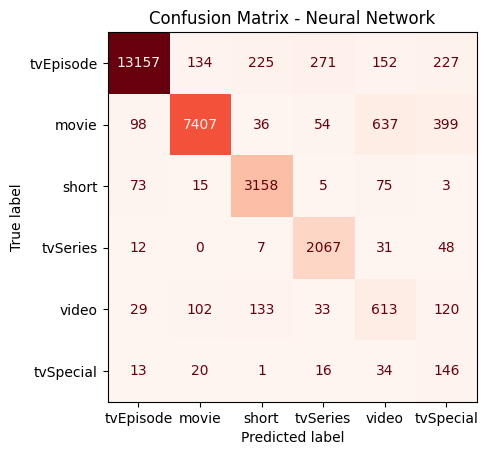
\includegraphics[width=\textwidth]{plotsss/cm_nn_titletype.png}
        \caption{Confusion Matrix - Neural Network}
        \label{fig:cm_nn_titletype}
    \end{subfigure}
    \hfill
    \begin{subfigure}[b]{0.52\textwidth}
        \centering
        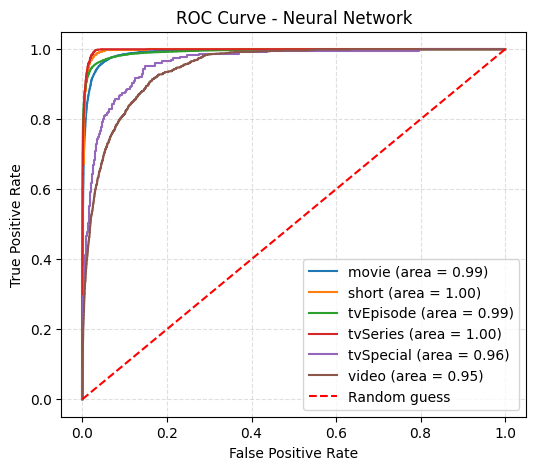
\includegraphics[width=\textwidth]{plotsss/roc_nn_titletype.png}
        \caption{ROC Curve - Neural Network}
        \label{fig:roc_nn_titletype}
    \end{subfigure}
    \caption{Confusion Matrix and ROC Curve for the Neural Network on the \texttt{titleType} classification task.}
    \label{fig:cm_nn_titletype}
\end{figure}




\subsection{Model Comparison}